\documentclass[tikz]{standalone}
\usetikzlibrary{shapes,arrows,positioning}
\usetikzlibrary{arrows.meta}

\begin{document}
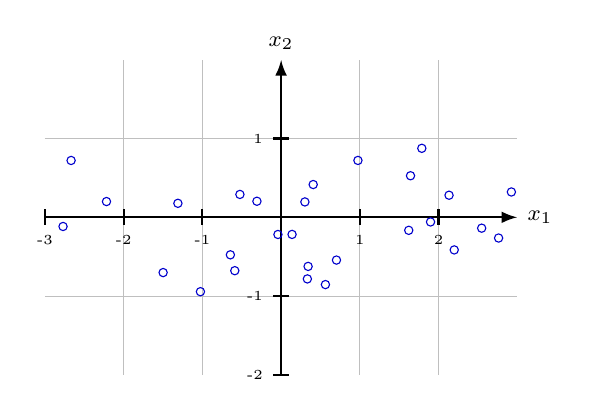
\begin{tikzpicture}

% Draw gridlines
   % Draw horizontal grid lines
    \foreach \y in {,-1,0,1} {
        \draw[gray!50, thin] (-3,\y) -- (3,\y);
    }

    % Draw vertical grid lines
    \foreach \x in {-2,-1,0,1,2} {
        \draw[gray!50, thin] (\x,-2) -- (\x,2);
    }

% X-axis with arrow and labeled ticks
\draw[thick,-{Latex[length=2mm]}] (-3,0) -- (3,0) node[right] {{\footnotesize $x_1$}};
\foreach \x in {-3,-2,-1,1,2}
  \draw[thick] (\x,0.1) -- (\x,-0.1) node[below] {{\tiny \x}};

% Y-axis with arrow and labeled ticks
\draw[thick,-{Latex[length=2mm]}] (0,-2) -- (0,2) node[above] {{\footnotesize $x_2$}};
\foreach \y in {-2,-1,1}
  \draw[thick] (0.1,\y) -- (-0.1,\y) node[left] {{\tiny \y}};

% Define and plot the points
\foreach \x/\y in {
  -1.02442/-0.944555, 1.78712/0.87635, -1.49814/-0.70177, 0.343144/-0.623502,
  -0.588122/-0.677732, 0.139294/-0.217198, 2.13292/0.280655, 0.562863/-0.854298,
  1.89802/-0.058724, -1.3107/0.177829, 2.76225/-0.263087, -0.306967/0.204073,
 -2.66687/0.72193, 2.92472/0.321828, -0.522994/0.290584,
  1.62113/-0.165155, 0.97585/0.722508, -2.76925/-0.116417, 0.407738/0.416384,
  0.302254/0.1954, 0.333625/-0.782259, -2.21745/0.200276,
  0.703271/-0.54302, 2.19896/-0.413959, 1.64372/0.527912, 2.5473/-0.137799,
  -0.644052/-0.476276, -0.0399483/-0.21801
} %Since most variation is in x_1 direction, we won't lose much variation if we project all data points onto x_1 and then consider this reduced data. However, it makes more sense to consider linear combinations of our data as the next example will show (the reason we take linear combinations is because we can account for correlation in x_1 and x_2. Because the variables are uncorrelated in this example, linear combinations are actually redundant)
%\foreach \x/\y in {
%  -1.02442/0, 1.78712/0, -1.49814/0, 0.343144/0,
%  -0.588122/0, 0.139294/0, 2.13292/0, 0.562863/0,
%  1.89802/0, -1.3107/0, 2.76225/0, -0.306967/0,
% -2.66687/0, 2.92472/0, -0.522994/0,
%  1.62113/0, 0.97585/0, -2.76925/0, 0.407738/0,
%  0.302254/0, 0.333625/0, -2.21745/0,
%  0.703271/0, 2.19896/0, 1.64372/0, 2.5473/0,
%  -0.644052/0, -0.0399483/0
%}
{
% Draw horizontal line to x-axis
%\draw[red!70!black, dotted, thick] (\x,0) -- (\x,\y);

% Draw the point
\draw[blue!80!black] (\x,\y) circle (1.5pt);
}

\end{tikzpicture}
\end{document}
